\documentclass{article}

\usepackage[french]{babel}
\usepackage[T1]{fontenc}
\usepackage{moreverb}       % verbatim with tab

\usepackage{wrapfig}
\usepackage{graphicx}
\usepackage{geometry}
\geometry{hmargin=2.5cm}
\usepackage{amsmath}
\usepackage{siunitx}

\usepackage{graphicx}
\usepackage{subcaption}
\usepackage{float}
\usepackage{hyperref}
\usepackage{setspace}
\usepackage{xcolor}
\usepackage{pdfpages}
\usepackage{enumitem}
\usepackage{lscape}

% https://tug.org/FontCatalogue/libertinusserif/
%\usepackage{libertinus}
%\usepackage[T1]{fontenc}

\usepackage{libertine} % Police Linux Libertine en sérif, Linux Biolinum en sans-sérif.

\usepackage[libertine]{newtxmath} % Math avec la police Libertine
%\addtokomafont{disposition}{\normalfont\sffamily} % Police des titres (ajouter \normalfont pour enlever le bold)
%\addtokomafont{paragraph}{\bfseries} % Titre des paragraphes en gras
%\addtokomafont{subsubsection}{\bfseries} % Titre des subsubsections en gras
%\usepackage[scaled=.8]{beramono} % Police monospace

\usepackage{fancyhdr}       % en-têtes
\usepackage{lastpage}       % numéro de dernière page

\usepackage{appendix}       % annexes

% code
\usepackage{xcolor}
\usepackage{listings}

\definecolor{mGreen}{rgb}{0,0.6,0}
\definecolor{mGray}{rgb}{0.5,0.5,0.5}
\definecolor{mPurple}{rgb}{0.58,0,0.82}
\definecolor{backgroundColour}{rgb}{0.95,0.95,0.92}

\lstdefinestyle{CStyle}{
    backgroundcolor=\color{backgroundColour},   
    commentstyle=\color{mGreen},
    keywordstyle=\color{magenta},
    numberstyle=\tiny\color{mGray},
    stringstyle=\color{mPurple},
    basicstyle=\footnotesize,
    breakatwhitespace=false,         
    breaklines=true,                 
    captionpos=b,                    
    keepspaces=true,                 
    numbers=left,                    
    numbersep=5pt,                  
    showspaces=false,                
    showstringspaces=false,
    showtabs=false,                  
    tabsize=2,
    language=C
}

\title{Développement d'un codec audio AAC : optimisation de l'algorithme MDCT pour une architecture ARM}
\date{2020 -- 2021}
\author{Laura Binacchi}

\pagestyle{fancy}
\renewcommand\headrulewidth{1pt}
\fancyhead[L]{Laura Binacchi}
\fancyhead[C]{Développement d'un codec audio AAC}
\fancyhead[R]{2021 -- 2022}

\AtBeginDocument{
    \def\labelitemi{\textbullet}    % Redéfinition des puces dans les itemize
    \renewcommand{\times}{\text{×}} % Remplacer le gros «X» par un plus beau
    %\interfootnotelinepenalty=10000
}

\lstset { %
    language=C++,
    backgroundcolor=\color{black!5}, % set backgroundcolor
    basicstyle=\footnotesize,% basic font setting
}

\begin{document}
    \pagenumbering{gobble}
    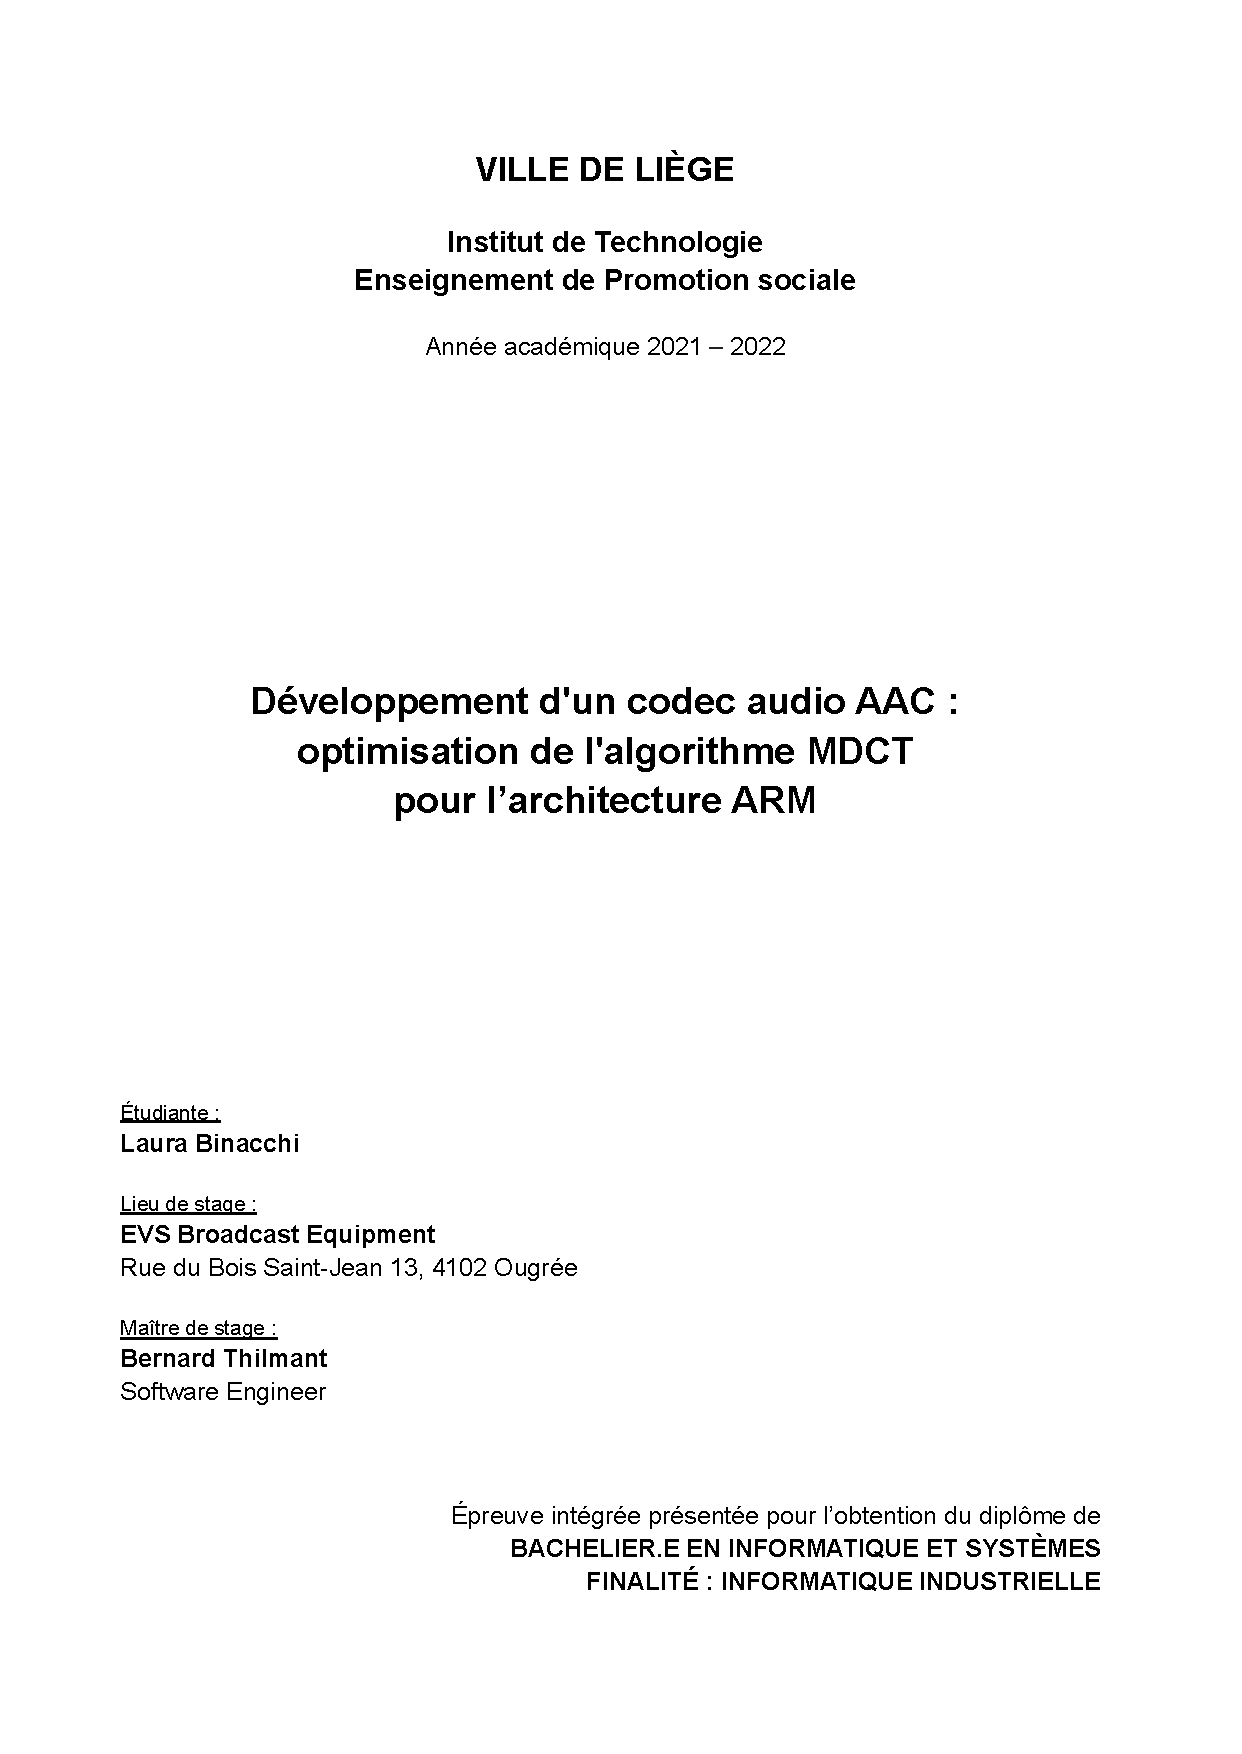
\includepdf[pages={1}]{pdg}
    \newpage
    \tableofcontents
    \newpage
    \pagenumbering{arabic}

    \section*{Remerciements}
    \paragraph{}

    \section*{Introduction}
    \addcontentsline{toc}{section}{\protect\numberline{}Introduction}

    % Contexte du projet : serveur XT (XT VIA qui succède à ...) et passage d'une architecture Intel à une architecture ARM
    % Travail qui s'inscrit dans la continuité d'un travail théorique préalable
    % Optimisations possibles et choix de l'algorithme MDCT (mais on pourrait aussi faire la même chose pour le bloc quantization, etc.)
    % Optimisations du bloc MDCT mises en place : passage d'une arithmétique floating à fixed point et utilisation des fonctions SIMD qui offrent une meilleur capacité de calcul
    % Limite de l'optimisation : limite de temps (temps du stage) plutôt que gain de performance par rapport à ce qui est déjà en prod

    \paragraph{}
    Développement d'une solution de software embarqué sur processeur ARM pour encodage audio AAC optimisé aux applications d'EVS :
    \begin{itemize}
        \item Prise de connaissance de l'encodage AAC et de l'environnement EVS qui utilise ce type de format ;
        \item Prise de connaissance des résultats des optimisations possibles du modèle psycho-acoustique développé par EVS ;
        \item Développement du code en C ou Assembler pour l'encodage AAC sur plateforme ARM ;
        \item Test du système et documentation de son implémentation.s possibles du modèle psycho-acoustique développé par EVS ;
        \item Développement du code en C ou Assembler pour l'encodage AAC sur plateforme ARM ;
        \item Test du système et documentation de son implémentation.
    \end{itemize}

    \paragraph{}
    %Mon travail s'inscrit dans la continuité de celui de Wafaa Heddari, stagiaire qui m'a précédée au sein du département hardware-firmware d'EVS pour y travailler sur le codec AAC. Après une étude du codec AAC et des différents blocs qui le composent, son mémoire dégage des pistes d'amélioration des performances du codec AAC : like Removal of block switching, Fast MDCT, and Optimized TNS. And then test their implementation on C Code to compare the compilation speed between the original Codec and the optimized one\cite{Wafaa}.

    %L'amélioration des performances est nécessaire par la qualité grandissante des données audio et video -> de plus en plus grandes, et le besoin de maintenir plusieurs flux en tant réel dans le broadcast

    \paragraph{}
    Ce travail commencera par une présentation d'EVS et du département dans lequel s'est déroulé mon stage. Parmi les nombreux produits d'EVS, seul le serveur XT sera brièvement présenté puisque c'est spécifiquement pour ce dernier que le codec AAC est développé et optimisé.

    \paragraph{}
    Quelques notions théoriques indispensables à la compréhension du travail pratique seront ensuite développées avec une section consacrée au son et sa numérisation et une autre consacrée aux codecs MPEG, à leur fonctionnement et en particulier au fonctionnement du bloc MDCT de l'encodeur AAC.

    % But : garder la max de performance en perdant le moins en qualité


    \newpage
    \section{EVS Broadcast Equipment}
    \subsection{Présentation d'EVS et du département R\&D}
    \paragraph{}
    Mon stage s'est déroulé au sein de la société EVS Broadcast Equipment dont la figure \ref{fig:logo} représente le logo. EVS est une entreprise d'origine liégeoise devenue internationale. Fondée en 1994 par Pierre L'Hoest, Laurent Minguet et Michel Counson, EVS compte aujourd'hui plus de 600 employés dans plus de 20 bureaux à travers le monde mais son siège principal se situe toujours à Liège.

    \begin{figure}[H]
        \centering
        
\includegraphics[width=.5\linewidth]{./images/EVS-logo.png}
        \caption{Logo de la société EVS Broadcast Equipment\cite{EVS:website}}
        \label{fig:logo}
    \end{figure}

    \paragraph{}
    EVS est devenu leader dans le monde du broadcast avec ses serveurs permettant l'accès et la diffusion instantanée des données audiovisuelles enregistrées sur ses serveurs. L'entreprise est également célèbre pour ses ralentis instantanés. Ces technologies sont utilisées pour la production live des plus importants événements sportifs dans le monde : le matériel EVS est notamment utilisé pour la retransmission des Jeux Olympiques depuis 1998.

    \paragraph{}
    Plus de 50\% des employés d'EVS travaillent en recherche et développement afin de répondre au marché du broadcast en constante évolution. Outre ses solutions techniques innovantes, EVS se différencie de ses concurrents par la proximité entretenue avec les clients en leur proposant des solutions à l'écoute de leurs besoins et en leur offrant un service de support de qualité.

    \paragraph{}
    C'est en R\&D, dans l'équipe Hardware-Firmware, que s'est déroulé mon stage. Sous la direction de Justin Mannesberg, cette équipe se compose d'une vingtaine d'employés spécialisés en développement embarqué et en développement FPGA. La situation particulière dans laquelle s'est déroulé mon stage, en pleine pandémie de Covid et alors que tous les employés étaient confinés, ne m'a pas permis d'interagir avec beaucoup de membres de l'équipe et ni de pouvoir observer leur travail. Bernard Thilmant (Software Engineer dans l'équipe Hardware-Firmare) a cependant réussi à m'apporter le soutien nécessaire à la bonne réalisation de mon stage : il m'a permis de m'initier au C++, m'a aidée à ne pas me perdre dans les concepts parfois complexes de l'encodage audio et m'a aidée à apporter la rigueur scientifique nécessaire à la réalisation de mon travail. J'ai également pu bénéficier de l'expertise technique de Frédéric Lefranc (Principal Embedded System Architect dans l'équipe Hardware-Firmare) ainsi que du suivi de Justin Mannesberg (Manager de l'équipe Hardware-Firmware).

    \subsection{Le serveur XT}
    \paragraph{}
    EVS développe et commercialise de nombreux produits allant des serveurs de production aux interfaces permettant d'exploiter des données audio-visuelles ou de monitorer des systèmes de production\cite{EVS:products}. Le serveur de production live XT est un des produits emblématiques d'EVS. Il permet de stocker de grandes quantités de données audio-visuelles et d'y accéder en temps réel afin de répondre aux besoins de la production en live. Par exemple, la remote LSM (\emph{Live Slow Motion} permet d'accéder aux contenus des serveurs XT afin de créer les ralentis pour lesquels EVS est célèbre dans le monde.

    \begin{figure}[H]
        \centering
        \begin{subfigure}[b]{0.4\linewidth}
            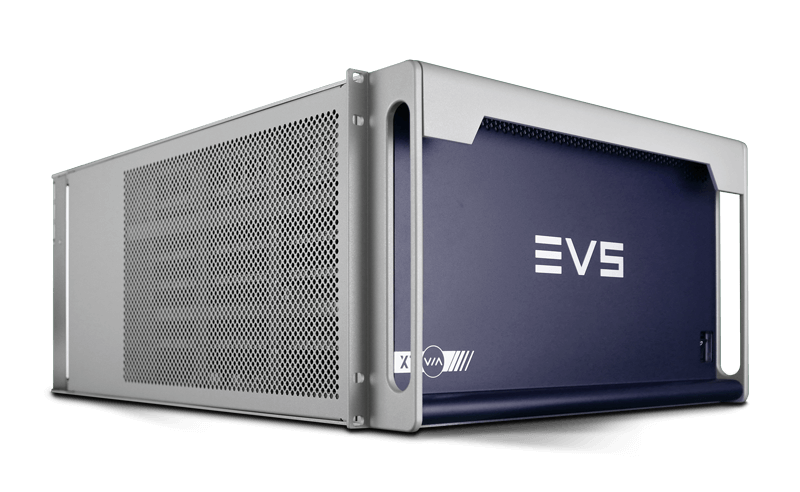
\includegraphics[width=\linewidth]{./images/XT-VIA.png}
        \end{subfigure}
        \begin{subfigure}[b]{0.4\linewidth}
            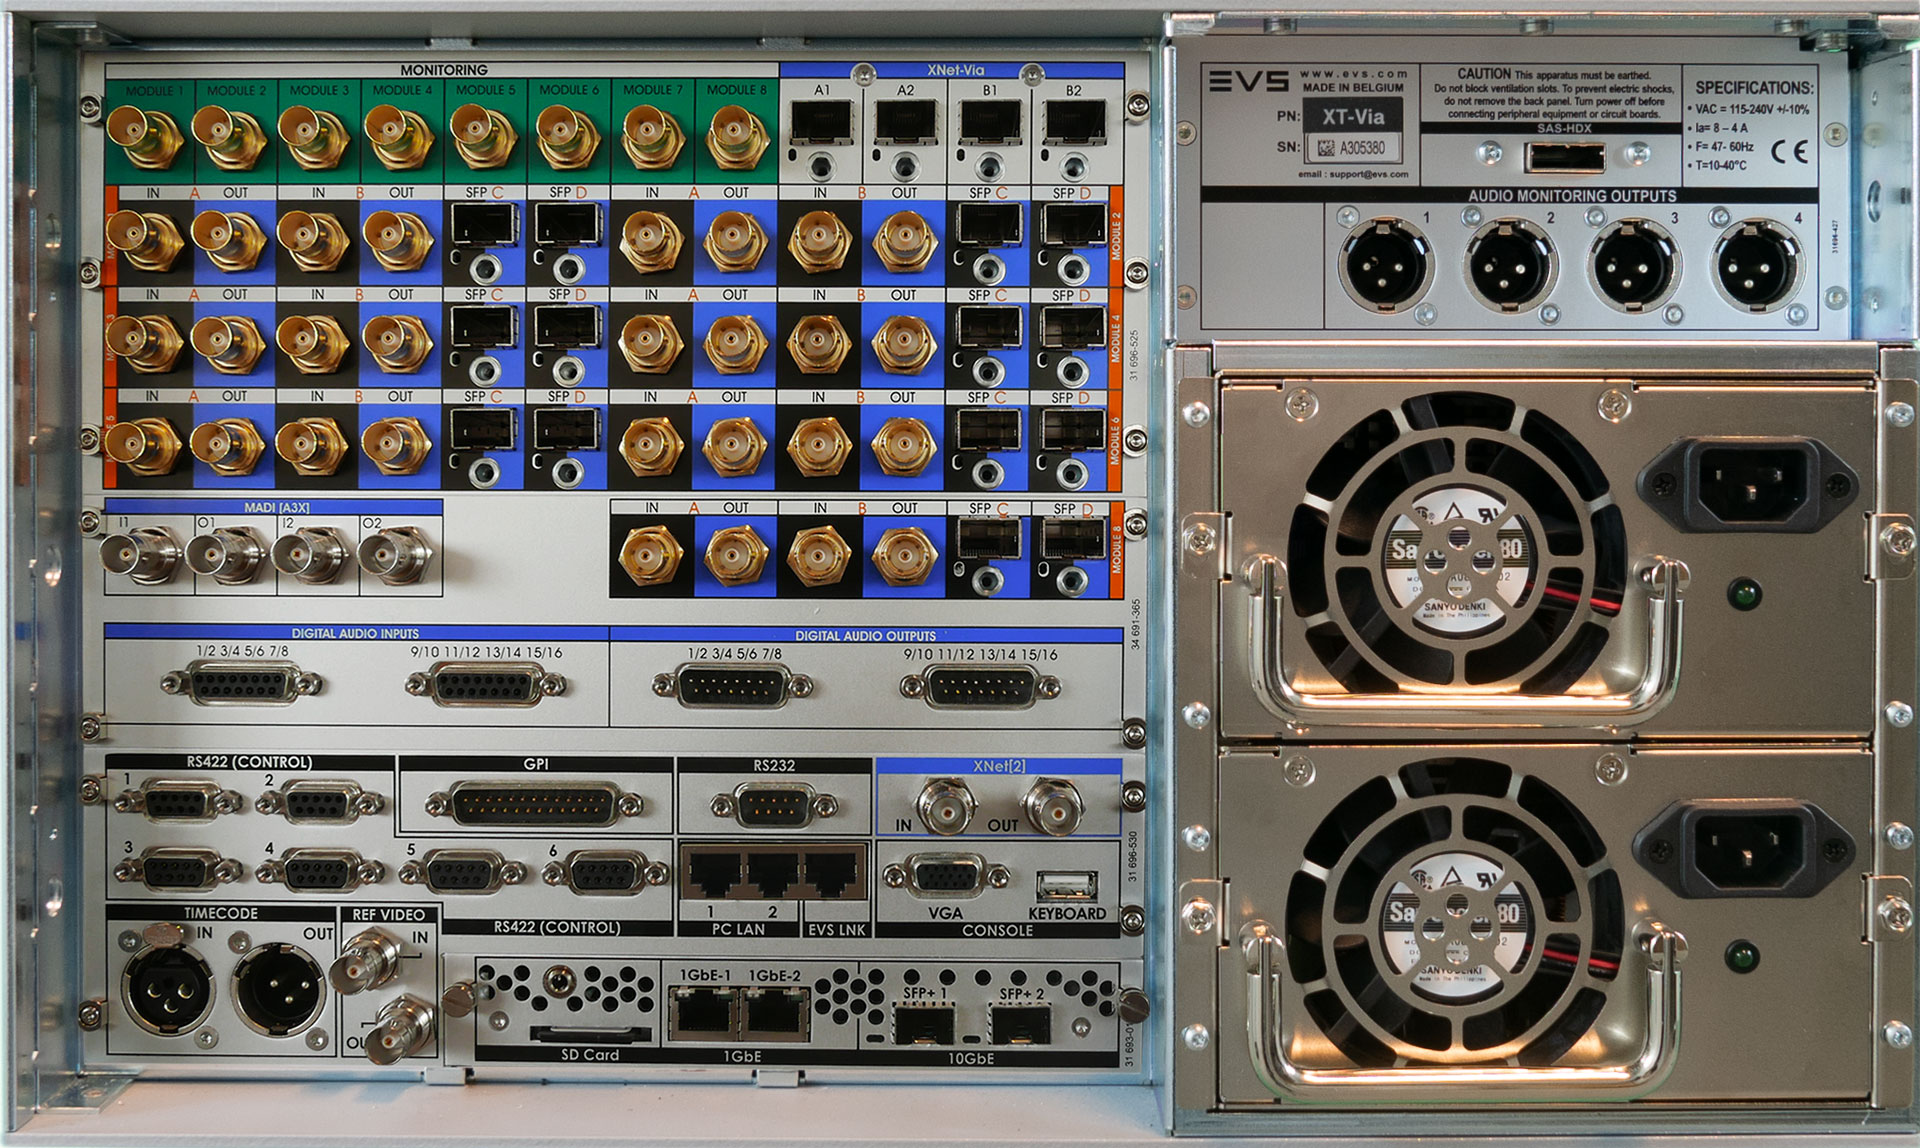
\includegraphics[width=\linewidth]{./images/XT-VIA-ar.jpg}
        \end{subfigure}
        \caption{Vues avant et arrière (en configuration IP) de l'XT-VIA\cite{EVS:products}}
        \label{fig:xt-via}
    \end{figure}

    \paragraph{}
    Le serveur XT a connu plusieurs versions : XT, XT2, XT2+, XT3 et enfin l'XT-VIA. L'XT-VIA (cf figure \ref{fig:xt-via}), la plus récente version du serveur XT, en quelques informations clés\cite{EVS:products} :
    \begin{itemize}
        \item offre un espace de stockage de 18 à 54 TB, soit plus de 130h d'enregistrement en UHD-4K;
        \item dispose de 2 à plus de 16 canaux selon le format choisi : 2 canaux en UHD-8K (4320p), 6 canaux en UHD-4K (2160p) et plus de 16 canaux en FHD and HD (720p, 1080i, 1080p);
        \item permet une configuration hybride de ses entrées et sorties en IP (10G Ethernet SFP+, 100G en option, ST2022-6, ST2022-7, ST2022-8, ST2110, NMOS IS-04, IS-05, EMBER+, PTP) ou SDI (1.5G-SDI, 3G-SDI et 12G-SDI);
        \item supporte de nombreux formats d'encodage vidéo : UHD-4K (XAVC-Intra et DNxHR), HD/FHD (XAVC-I, AVC-I, DNxHD et ProRes), PROXY (MJPEG et H264);
        \item peut enregistrer 192 audio tracks non compressés et supporte les standards AES et MADI;
        \item offre de nombreuses possibilités de connection avec du matériel EVS ou non.
    \end{itemize}

    \paragraph{}
    C'est pour la dernière génération du serveur XT, l'XT-VIA, que le codec AAC est développé. La compression avec perte de données de ce codec permet d'optimiser l'espace occupé par les données audio sans en altérer la qualité perçue. Outre la qualité audio, les performances de l'encodage sont importantes à prendre en compte pour permettre l'enregistrement de plusieurs canaux en parallèle tout en conservant un traitement de l'information qui tienne le temps réel. L'optimisation des performances doit tenir compte de l'architecture de l'XT-VIA : l'architecture ARM Neon remplace l'architecture Intel x86 de ses prédécesseurs avec des différences importantes dans les fonctions intrinsèques.


    \newpage
    \section{L'encodage audionumérique : généralités}
    \subsection{Le son}
    % onde acoustique -> 

    % - son audible = vibration entre 20 et 20kHz

    % le signal, analogique (continu) ou discret, peut avoir une représentation :
    % - temporelle
    % - fréquentielle
    % exemple de signaux périodiques (sinus, carré, etc) -> pp 6-7 + truc interactif

    % - spectre d'amplitude (utile) et spectre de phase (pas utile)

    % - toute fonction p(x, t) peut être exprimée par une somme de fonctions (co-)sinusoidales : formule pour les fonctions périodiques + transformée de Fourier pour les fonctions n'est pas périodique dans le temps

    \subsection{La numérisation d'un signal}
    \label{audionumerique}
    % transformation de fourier :
    % https://www.claudegabriel.be/Math%C3%A9matiques%20appliqu%C3%A9es,%20chapitre%204.pdf -> p12 sur N pair / impair
    % à la base -> signaux périodique (faire bref)
    % -> ce qui nous intéresse : transformation pour signal non périodique discret -> DCT


    \newpage
    \section{Les codecs audio}
    \subsection{Définition d'un codec}
    \paragraph{}
    Un codec est un procédé logiciel composé d'un encodeur (\emph{\textbf{co}der}) et d'un décodeur (\emph{\textbf{dec}oder})\cite{wiki:codec}. Un codec audio permet donc, d'une part, de coder un signal audio dans un flux de donnée numériques et, d'autre part, de décoder ces données afin de restituer le signal audio.

    \paragraph{}
    Les codecs sont dits avec perte (\emph{lossy}) ou sans perte (\emph{lossless}). Le PCM est par exemple un codec sans perte puisqu'il encode la totalité des informations sonores dans la bande de fréquences humainement audible. Ce type de codec permet de conserver la qualité de l'audio mais nécessite en contrepartie un espace de stockage conséquent, même avec une compression des données.

    \paragraph{}
    Afin de réduire l'espace de stockage nécessaire, les codecs avec perte permettent de supprimer une partie des données audio. C'est le cas des codecs définis par les normes MPEG dont fait partie le codec AAC.

    \subsection{Les codecs MPEG}
    \paragraph{}
    MPEG (\emph{Moving Picture Experts Group}) désigne une alliance de différents groupes de travail définissant des normes d'encodage, de compression et décompression et de transmission de média audio, vidéo et graphiques\cite{wiki:MPEG}. Le groupe est actif depuis 1988 et a produit depuis de nombreuses normes.

    \paragraph{}
    Les codecs audio qui implémentent les normes MPEG ont pour point commun d'être des codecs avec perte de données basés sur un modèle psychoacoustique. Le premier est le MP3, défini par la norme MPEG-1 Layer-3 ISO/IEC 11172-3:1993. Le codec AAC est conçu en 1997 pour remplacer le MP3. Il est défini par les normes MPEG-2 partie 7 ISO/IEC 13818-7:2006\cite{ISO13818-7} et MPEG-4 partie 3 ISO/IEC 14496-3:2019\cite{ISO14496-3}.

    \paragraph{}
    Les normes MPEG définissent les grandes lignes de l'encodage et du décodage et le format du conteneur mais pas l'implémentation du codec qui peut de ce fait être plus ou moins performant. Les codecs MPEG sont typiquement composés des blocs suivants :
    \begin{figure}[H]
        \centering
        \begin{subfigure}[b]{.6\linewidth}
            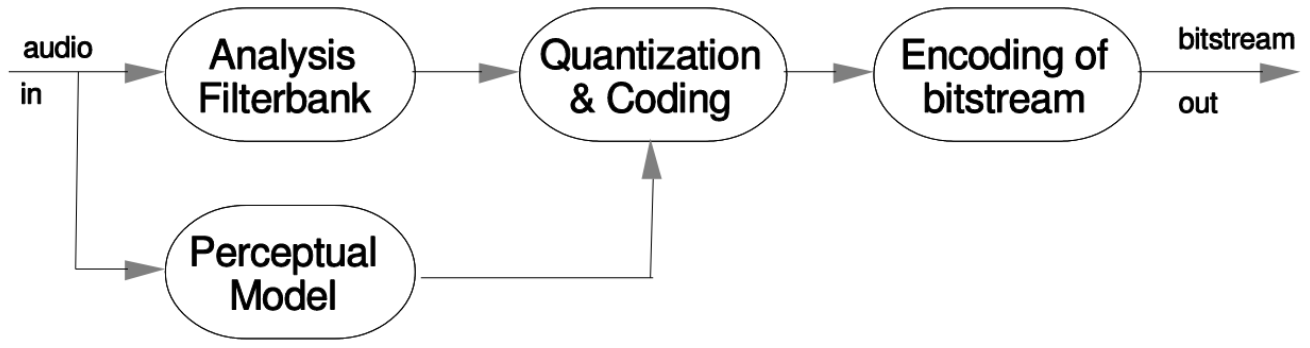
\includegraphics[width=\linewidth]{./images/1999-Brandenburg-simple-AAC-encoder.png}
            \caption{Schéma fonctionnel de l'encodeur}
        \end{subfigure}
        \begin{subfigure}[b]{.6\linewidth}
            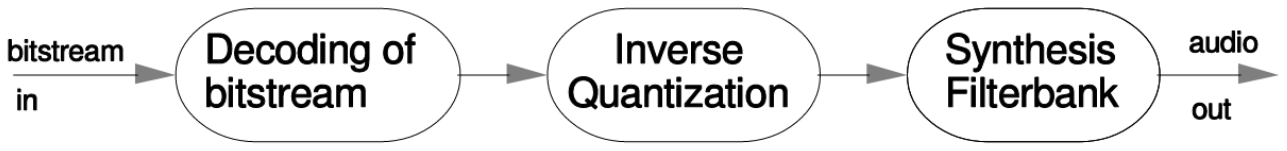
\includegraphics[width=\linewidth]{./images/1999-Brandenburg-simple-AAC-decoder.png}
            \caption{Schéma fonctionnel du décodeur}
        \end{subfigure}
        \caption{Vue simplifiée d'un codec MPEG basé sur un modèle psychoacoustique\cite{1999-Brandenburg}}
    \end{figure}
    \paragraph{}
    L'encodeur est composé des blocs suivants :
    \begin{description}
        \item[filter bank] la banque de filtres décompose le signal temporel d'entrée en différentes composantes fréquentielles
        \item[perceptual model] le modèle psychoacoustique utilise le signal temporel et/ou sa décomposition fréquentielle pour éliminer les données audio dont l'absence ne nuira pas à la qualité perçue à l'écoute ()
        \item[quantization and coding] la quantification attribue une valeur numérique aux données du spectre de fréquences : elle sont typiquement codées avec une méthode entropique qui peut être optimisée avec le modèle psychoacoustique
        \item[encoding of bitstream] les données sont formatées en un flux contenant typiquement le spectre de fréquences codé et des informations supplémentaires permettant l'encodage
    \end{description}
    
    \paragraph{}
    Le décodeur a un fonctionnement inverse : le flux de données est décodé (\textbf{decoding of bitstream}), les composantes fréquentielles du signal sont retrouvées par l'opération inverse à la quantification (\textbf{inverse quantization}) et ces sous-bandes fréquentielles sont finalement rassemblées pour reconstituer le signal temporel (\textbf{synthesis filter bank}).

    \paragraph{}
    Le fonctionnement du décodeur ne sera pas plus développé dans ce travail car le bloc MDCT fait partie de la banque de filtres de l'encodeur. Le fonctionnement spécifique de l'encodeur AAC sera par contre détaillé dans la section \ref{sec:AAC}.


    \subsection{Les modèles psychoacoustiques}
    \paragraph{}
    Le section précédente a défini les codecs MPEG comme étant basés sur un modèle psychoacoustique. La psychoacoustique est une branche de la psychophysique qui étudie la manière dont l'oreille humaine perçoit le son\cite{wiki:psychoacoustic}. Cette discipline permet d'améliorer la compression d'un signal audio en éliminant les sons qui sont captés par un microphone mais qui ne peuvent pas être perçus par l'oreille humaine et les avancées dans cette discipline permettent de développer des encodeurs audio de plus en plus performants. Les codecs basés sur un modèle psychoacoustique sont toujours des codecs avec perte puisqu'une partie des informations auditives sera définitivement perdue, ce qui ne nuit pour autant pas à la qualité perçue du son.

    \paragraph{}
    L'encodage audionumérique tient déjà compte des seuils de fréquences humainement audibles pour limiter les données audio enregistrées : nous l'avons vu dans la section \ref{audionumerique}, aucun son n'est perçu en-deça de 20Hz ou au-delà de 20kHz. La psychoacoustique permet de mieux dessiner limite entre ce qui est humainement audible ou non afin d'éliminer un maximum des informations non pertinentes et ainsi augmenter le facteur de compression des données : le facteur de compression des codecs MPEG est environ 15 fois supérieur à celui du CD\cite{2019-Herre-Dick}.

    \paragraph{}
    Les effets de masque sont au centre des différents modèles psychoacoustiques utilisés pour la compression audio. L'enjeu afin d'obtenir le meilleur taux de compression est de calculer le plus finement possible les seuils de masquage, i.e. la limite entre les informations pertinentes et celles qui peuvent être éliminées. Les effets de masques dans le domaine fréquentiel (\emph{spectral masking effects}) sont parmi les plus utilisés mais il en existe d'autres, e.g. dans le domaine temporel. La figure suivante représente différents effets de masque du domaine fréquentiel :
    \begin{figure}[H]
        \centering
        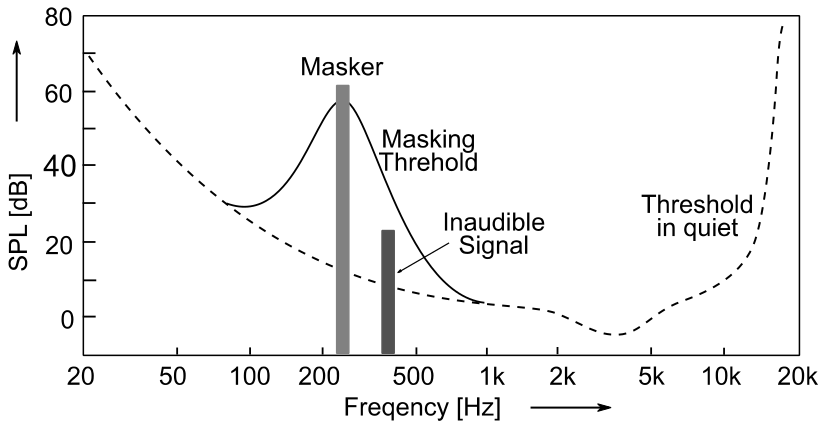
\includegraphics[width=.6\linewidth]{./images/2019-Herre-Dick-masking-effect.png}
        \caption{Effets de masque dans le domaine fréquentiel\cite{2019-Herre-Dick}}
    \end{figure}

    \paragraph{}
    Les lignes représentent le seuil 
    \begin{description}
        \item[Threshold in quiet] la ligne en pointillé représente le seuil d'audibilité dans le calme, indépendamment de tout autre élément qui pourrait interférer
        \item[Masking threshold] 
    \end{description}


    % SPL) A frequency dependent threshold of in hearing in quiet describes the minimum sound pressure level of a sound to be perceivable isolation and under extremely quite conditions. (SPL) of a sound be perceivable in isolation and curve under extremely conditions. • In the presence of to a masker, the threshold in quiet changes into quite a masking threshold, which bell-shaped increase the in frequencies the vicinity of the masker, depending on its • shows In the a presence of a masker, threshold in in quiet curve changes into a masking threshold, frequency, level, and signal increase type. Any sound beneath threshold is masked by the louder which shows a bell-shaped in frequencies in the this vicinity of the masker, depending on its signal, and level, thus and inaudible the Any average perceptual coding, the louder coding signal, error frequency, signal for type. sound listener. beneath In this threshold audio is masked by the (i.e., the introduced quantization noise) corresponds to the probe signal in this experimental and thus inaudible for the average listener. In perceptual audio coding, the coding error (i.e., scenario. the introduced quantization noise) corresponds to the probe signal in this experimental scenario. • Masking effects are are strongest strongest signals are within the critical bandwidth of the masker. • Masking effects for for signals that that are within the critical bandwidth of the masker. Within Within the critical bandwidth, the masking threshold remains constant. Furthermore, the the critical bandwidth, the masking threshold remains constant. Furthermore, the masking effects masking spread to frequencies the (so-called critical bandwidth (so-called The inter-band spread to effects frequencies beyond the critical beyond bandwidth inter-band masking). upper masking). The upper slope of the masking threshold depends on multiple factors, such as absolute slope of the masking threshold depends on multiple factors, such as absolute frequency and sound frequency and of sound pressure whereas level of the the lower masker, whereas lower slope dependency. hardly shows a level pressure level the masker, slope hardly the shows a level dependency. • Depending on the type of masker, i.e., tone or (narrow-band) noise, the strength of the masking • Depending the type of masker, i.e., can tone or (narrow-band) the strength of the masking effect varies. on While noise-like maskers mask tone-like signals noise, very well (up to a masker-to-probe effect varies. maskers can mask tone-like signals very well (up to a masker-to- level ratio of While about noise-like 6 dB), tone-like maskers can mask noise only to a much weaker extent [29] probe level ratio of about 6 dB), tone-like maskers can mask noise only to a much weaker extent (about 20 dB). [29] (about 20 dB).      \paragraph{}     Le calcul des   


    
    
    
    Le calcul du seuil de masquage tient compte\cite{2019-Herre-Dick} :
    \begin{itemize}
        \item des effets de masquage monophonique de la perception non-linéaire des fréquences, plus fine pour les basses fréquences;
        \item des effets de masque dans le temps;
        \item de l'effet de masque dans une bande de fréquence ou entre bandes de fréquences;
        \item l'impact de la tonalité sur le masquage
        \item masking over time
    \end{itemize}


    \newpage
    \section{Le codec AAC}
    \label{sec:AAC}
    \subsection{Fonctionnement de l'encodeur AAC}
    % présentation des différents blocs
    % \cite{wiki:AAC}

    %In this thesis, we are going to study the different blocks of an AAC encoder based on the standard ISO/IEC 13818-7 such as the psychoacoustic model, Gain control, Transform block, Spectral processing, Quantization and Entropy coding. \cite{Wafaa}

    % Les codecs définis par les normes MPEG sont basés sur le modèle psychoacoustiquev
    % Les performances des codecs audio définis par les normes MPEG sont rendues possibles par les recherches en psychoacoustique.


    %AAC supports inclusion of 48 full-bandwidth (up to 96 kHz) audio channels in one stream plus 16 low frequency effects (LFE, limited to 120 Hz) channels, up to 16 "coupling" or dialog channels, and up to 16 data streams. The quality for stereo is satisfactory to modest requirements at 96 kbit/s in joint stereo mode; however, hi-fi transparency demands data rates of at least 128 kbit/s (VBR). Tests[which?] of MPEG-4 audio have shown that AAC meets the requirements referred to as "transparent" for the ITU at 128 kbit/s for stereo, and 320 kbit/s for 5.1 audio.[citation needed] 
    % AAC uses only a modified discrete cosine transform (MDCT) algorithm, giving it higher compression efficiency than MP3, which uses a hybrid coding algorithm that is part MDCT and part FFT.[4]


    \paragraph{}
    Le codec AAC (Advanced Audio coding) est définit  , défini par la norme . Les recherches en psychoacoustique ont permis de développer un algorithme d'encodage plus performant pour l'AAC que pour le MP3 : il permet d'encoder moins données audio tout en gardant la même qualité perçue au décodage\cite{1999-Brandenburg}.



    \subsection{Le bloc MDCT}
    % \begin{itemize}
    %     \item particularités par rapport à la FFT
    %     \item basée sur la DCT-IV
    %     \item niveaux de complexité (O...)
    % \end{itemize}


    \newpage
    \section{Algorithmes MDCT de référence}
    \subsection{Description mathématique}
    \label{sec:desc-math}
    \paragraph{}
    La transformation effectuée par la MDCT est donnée par l'équation suivante\cite{wiki:MDCT} :
    $$X_k = \frac{2}{\sqrt{2N}} \sum_{n=0}^{2N-1} x_n \cos \left[ \frac{\pi}{N} \left( N + \frac{1}{2} + \frac{N}{2} \right) \left( k + \frac{1}{2} \right) \right]$$
    \begin{description}
        \item[$X_k$] avec $k \in [0, N[$ pour une fenêtre d'entrée de 2N échantillons
        \item[$x_n$] avec $n \in [0, 2N[$ : la fenêtre d'entrée
        \item[$F: R^{2N} \rightarrow R^N$] la MDCT est une fonction linaire qui pour 2N nombres réels d'entrée produit N nombre réels en sortie
    \end{description}

    \paragraph{}
    La MDCT a été implémentée avec une fenêtre d'entrée de $2N = 1024$ échantillons. Le bloc de sortie, i.e. le spectre de fréquences de la fenêtre d'entrée, aura donc une taille de 512. Ces différentes valeurs, utilisées à de très nombreux endroits du code sont rassemblées dans le header \texttt{mdct\_constants.h} présenté dans l'annexe \ref{an:mdct_const}.

    \paragraph{}
    La section suivante présente deux implémentations simples de cette formule. Ces implémentations ne pourraient pas être utilisées sans avoir été optimisées car elles seraient beaucoup trop lentes pour un codec qui doit tenir le temps réel. La complexité d'une implémentation de cette formule est de $O(N^2)$ opérations (où N est la taille de la fenêtre d'entrée). Cette complexité peut être ramenée à $O(N \log N)$ opérations par une factorisation récursive. La complexité peut également être diminuée en se basant sur une autre transformation, e.g. une DFT (\emph{Discrete Fourier Transorm}) ou une autre DCT (\emph{Discrete Cosine Transform}) : la complexité sera alors de $O(N)$ opérations de pré et post processing en plus de la complexité de la DFT ou de la DCT choisie\cite{wiki:MDCT}. C'est cette dernière option qui a été retenue pour ce travail.

    \subsection{Algorithmes développé et utilisation}
    \paragraph{}
    La formule mathématique de la MDCT donnée à la section \ref{sec:desc-math} a été implémentée très simplement en algorithmique flottante avec la possibilité d'obtenir le spectre de fréquences codés en \emph{float}, \emph{double} ou \emph{int32} depuis une fenêtre d'entrée en \emph{int16}. L'objectif de cet implémentation est de pouvoir vérifier les données des implémentations optimisées de la MDCT et de mesurer leur précision.

    \paragraph{}
    La première implémentation de l'équation de la MDCT est présentée dans l'annexe \ref{an:ref_float_mdct}. La fonction développée permet de faire ses calculs et d'obtenir un résultat aussi bien en \emph{float}) (32 bits) qu'en \emph{double} (64 bits) grâce à l'utilisation d'un \emph{template}.

    \paragraph{}
    La seconde fonction de référence est présentée dans l'annexe \ref{an:ref_int_mdct}. Elle permettra de vérifier les résultats des implémentations optimisées en \emph{fixed point}. Tous les calculs ne sont pas fait en algorithmique entière : la fonction fait les mêmes calculs que la fonction de référence en algorithmique flottante (uniquement en \emph{double} cette fois garder le plus de précision possible) et cast le résultat final dans un integer de 32 bits qui correspond à une notation Qx.15 signée.

    \subsection{Validation}

    \paragraph{}% TODO
    Validation avec un code d'exemple qui correspond à un signal sinusoidal (single tone) -> annexes : génération d'un signal single tone + code qui sort les données.

    \paragraph{}% TODO
    Présentation des résultats sous forme de données brutes ou de graphique.

    \paragraph{}% TODO
    Explication de la lecture des résultats, calcul des bandes de fréquences représentées. Mise en évidence qu'on a bien une seule composante fréquentielle comme attendu pour un signal single tone

    \paragraph{}% TODO
    + les résultats auraient été plus précis avec la fonction de fenêtre -> voir améliorations possibles


    \newpage
    \section{Algorithme MDCT basé sur la FFT}
    \subsection{Optimisations attentues}
    % algo qui vient du code d'exemple dsprelated, basé sur la FFT
%    \url{https://infoscience.epfl.ch/record/59946}
%    \url{https://www.cis.rit.edu/class/simg716/Gauss_History_FFT.pdf}
%    \url{https://sci-hub.se/https://www.jstor.org/stable/29775194#}

    %jouer sur la symétrie pour ne calculer que la moitié

    % \subsection{Code DSP related}
    % Code qui se base sur une FFT avec opérations de pre et de post twiddle
    % Annexes : code de la MDCT, test et procédure d'installation de la librairie FFTW

    % au code de base, il faut aussi ajouter la fonction de fenêtre (MLT) qui n'était pas présente.
    \paragraph{}
    Choix de l'optimisation de la MDCT basé sur sur une DCT : la FFT -> complexité de O (N log N) (N taille de la fenetre) + O(N) opérations de pré et de post processing.

    \paragraph{}
    But : utiliser une FFT déjà optimisée pour n'avoir à optimiser "que" les opérations de pré et de post processing
    Exemple trouvé sur le site DSP related -> Annexe ? Citation ?

    \subsection{Implémentation de la MDCT basée sur la FFT de la librairie FFTW3}
    \paragraph{}
    Code développé à partir de cet exemple en annexe. Il est basé sur la librairie FFTW3 qu'on ne peut pas garder car ne permet pas de travailler en integer -> sera amené à être retravaillé.

    \paragraph{}
    Explications des paramètres du code :
    \begin{itemize}
        \item fenêtre de 1024
        \item pre-twiddle -> 256
        \item FFT => FFT avec une fenêtre d'entrée réduite et donc une complexité réduite
        \item post-twiddle -> 512
    \end{itemize}

    % \subsection{Réduction de la fenêtre d'entrée}
    % (pre et post processing/twiddles pour faire moins de FFT) -> réduction de la fenêtre de la FFT

    \subsection{Validation}
    \paragraph{}
    Validé avec un single tone signal + l'algo de référence.

    \paragraph{}
    Code d'exemple qui teste l'algo de référence et l'algo FFTW3 avec les mêmes données d'entrée pour comparaison. (on fait la différence pour la précision ? ce n'est peut être pas pertinent de la faire déjà)

    \paragraph{}
    Présentation des résultats sous forme de données brutes ou de graphiques.


    \newpage
    \section{Utilisation de la librairie Ne10}
    \subsection{Choix de la librairie}
    \paragraph{}
    Changement obligatoire car la FFT de FFTW3 est uniquement dispo en algo flottante et on veut une implémentation en fixed point.
    % Le code de dsp related faisait appel à la librairie FFTW mais elle ne propose pas de FFT en fixed point => Ne10 qui propose une FFT fixed point optimisée pour ARM (avec ou sans instructions Neon)

    \paragraph{}
    Librairie optimisée pour l'architecture ARMv8. Mais a aussi des implémentation plain C (intéressant car permet de mesurer la diff de perf entre les 2).

    \subsection{Implémentation de la MDCT basée sur la FFT Ne10 en arithmétique \emph{floating point}}
    \paragraph{}
    Explications de l'algo en annexe


    \section{Algorithme MDCT en arithmétique fixed point}
    \subsection{Arithmétique fixed point}
    \paragraph{}
    trivial en float (reprendre le code de dsp) mais pour l'implémentation en arithmétique entière, attention à mettre dans les bonnes ranges
    % \paragraph{Points d'attention}
    % \begin{itemize}
    %     \item les dépassements : 16 bits + 32 bits -> potentiellement 33 bits, 16*16 -> 32, etc. à voir en fonction des valeurs réelles
    %     \item alignement des tableaux (souvent c'est une contrainte imposée car permet facilement d'optimiser du code) : résolutions possibles en allouant dynamiquement les tableaux et en jouant avec une arithmétique de pointeur OU utilisation de posix mem align...
    % \end{itemize}

    % Attention à la manière d'écrire le code. Ici on n'a pas besoin de faire attention à ce que le compilateur puisse faire du inline (ex remplacer l'appel à z = add(a, d) par z = a+d pour économiser le call) car l'algo est déjà très optimisé -> pas d'optimisations de compilateur possible et en plus on a une grosse routine -> économiser un call n'est pas forcément intéressant.

    \subsection{Améliorations attendues}
    \paragraph{}
    Le code de DSP related est en floating point -> passage en fixed point : opérations sur des entiers plus performantes + meilleure intégration (éviter le passage artificiel de l'entier au flottant et inversement)
    % Sur le format Qx.y :
    % https://www.pathpartnertech.com/representing-decimal-data-in-q-format/
    % https://www.allaboutcircuits.com/technical-articles/fixed-point-representation-the-q-format-and-addition-examples/
    % https://en.wikipedia.org/wiki/Q_(number_format)
    % et surtout https://web.archive.org/web/20171104111827/http://www.superkits.net/whitepapers/Fixed%20Point%20Representation%20%26%20Fractional%20Math.pdf

    % Intérêt de passer un integer: même si on ne gagne que 5\% de performance, on gagne du temps avant (les données qu'on reçoit sont en int16 -> pas de conversion vers le float après) et après (la quantification notament sera probablement plus rapide en integer)

    % Test de performance : il faut qu'à la fin l'implementation fixed point soit au moins aussi rapide que floating point


    \subsection{Implémentation de la MDCT basée sur la FFT Ne10 en arithmétique \emph{fixed point}}
    \paragraph{}
    Explication du code en annexe en accord avec les explications de la première subsection sur le fixed point

    \subsection{Performances}
    \paragraph{}
    Explication du code en annexe qui permet de mesurer les performance (avec code Timer)

    \paragraph{}
    Démonstration des résultats

    \paragraph{}
    Explication des résultats pas attendus : à ce niveau, résultats pas intéressants car + d'opérations qu'en flottant et ARM a des fonctions d'algo flottante

    \paragraph{}
    Pour soutenir cette hypothèse :  Test de la librairie et des performances des différentes FFT : performances équivalentes en 32 bits (floating ou fixed) et deux fois plus rapides en 16 bits




    \subsection{Arithmétique fixed point}
 

    % Pas trop de C++ parce que faire un objet avec plein d'accessors, ce n'est pas très optimisé (on se retrouve avec un gros objet avec plein de variables). Derrière on fait de l'assembleur => il y a un trop grand écart. D'habitude les codesc audio sotn codés en C mais c'est aussi peut-être juste pour une raison historique.



    \section{Optimisations à l'architecture ARM}
    \subsection{Spécificités de l'architecture ARMv8}
    \paragraph{}
    Globalement reprend les tutos ARM
    % FFT déjà optimisées pour Neon mais limitations sur ce qui entre et ce qui sort
    % \subsubsection{FFT de la librairie Ne10}

    \subsection{Utilisation des fonctions Neon SIMD (intrinsic)}
    % \begin{itemize}
    %     \item voir la doc de neon \url{https://developer.arm.com/documentation/dht0002/a/Introducing-NEON/What-is-SIMD-/ARM-SIMD-instructions}
    %     \item voir comment faire ce qui doit être fait en fonction des instructions SIMD dispo : souvent il faut ranger correctement, splitter les registres correctement
    %     \item utilisation des instructions intrinsèques de GCC \url{https://fr.wikipedia.org/wiki/Fonction_intrins%C3%A8que}
    % \end{itemize}

    \paragraph{}
    Les opérations SIMD permettent de faire plusieurs opérations en une fois où l'algo normal n'en fait qu'une à la fois. L'algo SIMD permet de faire plusieurs modifications à la fois -> il faut ranger les données de manière à pouvoir l'appliquer facilement (fonction fenêtre -> tri des données ? )


    \paragraph{}
    Plus les données sur lesquelles on travaille sont petites, plus on peut faire d'opérations en parallèle -> il faut voir si la perte de précision est ok. -> mettre une représentation graphique, c'est beaucoup plus simple à comprendre. D'où l'intérêt de passer à du 16 bits, plutôt que de rester en 32 bits et il faut absolument éviter le 64 bits (aucun intérêt).


    \section{Résultats}
    \subsection{Protocole de validation}
    %Validation aux différentes étapes des données : validation de la FFT, etc

    % \begin{itemize}
    %     \item sortie des données et générations de graphiques avec gnuplot
    %     \item résolution en fréquence pour une fenetre de 1024 samples pour un signal échantillonné à 48kHz : sur les graphiques $\frac{48000}{1024} = \SI{46.875}{\hertz}$ 1.3333... ms -> f = 1 / 1.33333 = 750 Hz OU res = fs / samples -> sur les graphiques on a des raies de fréquence de 750 Hz. Pour une fenêtre de 1024 = Hz
    % \end{itemize}
    % Graphiques sur sinusoide simple : augmenter la fréquence (i * qch pour déplacer la bande de fréquence), 

    %     Réaliser une fonction qui calcule la somme des cosinus (formule de wikipedia) pour chaque samples (pas du tout optimisée donc super lente). Pour la calcul en integer, on peut autoriser un manque de précision de max 1 LSB.


    % \begin{itemize}
    %     \item Voir les normes de test et règles d'acceptance des DCT et IDCT
    % \end{itemize}
    
    % \paragraph{}
    % Quand est-ce que la MDCT est assez optimisée ? Ici pas de critère de fin type 50 5 ou 2,5 \% plus rapide car pas de comparaison possible avec ce qui est actuellement en prod.

    % \paragraph{}
    % Pour les codecs c'est important de garder l'implémentation de référence mais à un moment on ne peut plus tester sur l'architecture intel. En pratique on utilise des pointeurs de fonction à déréférencer pour appeler l'implémentation voulue. En fonction du CPU ID, on sait quelles instructions on utilise. Au runtime, on choisit une ou l'autre implémentation en fonction de l'architecture, e.g. certains ARM n'ont pas les routines NEON



    \subsection{Gain en performance}
    % Comparaison avec un implémentation de référence plain c mais aussi à titre indicatif avec l'algorithme de référence car le plain c est déjà optimisé


    % L'impact de la window function : exemple avec un sinus : les composantes fréquentielles du sinus ressortent beaucoup mieux.

    % +difficultés au niveau des performances pas bonnes jusqu'à la fin

    \subsection{Perte de précision}
    % Comparaison avec l'algorithme de référence
    % Annexe : algo de référence, test de comparaison, résultats avec des données aléatoires et avec un sinus simple

    \newpage
    \section{Améliorations possibles}
    \begin{itemize}
        \item Fonction fenêtre intégrée aux opérations de pre twiddling
        \item Quantification intégrée au post twiddling
    \end{itemize}
    % Améliorations encore possible : faire les premières opérations de prétwiddling en Q15 8 par 8 avant de splitter, mêler les facteurs de la fenêtre aux facteurs de twiddling


    % DIFFICULTES
    % - calculs en Qx.x
    % - implémentation avec Ne10 car format de sortie, headroom et autres infos utiles pas documentées

    \newpage
    \section*{Conclusion}
    \addcontentsline{toc}{section}{\protect\numberline{}Conclusion}
    % Résultats obtenus + améliorations possibles

    \bibliography{biblio} 
    \bibliographystyle{ieeetr.bst}
    \addcontentsline{toc}{section}{\protect\numberline{}Références}
    
    \newpage
    \section*{Annexes}
    \begin{appendix}
        \section{Valeurs constantes utilisées dans le code}
        \label{an:mdct_const}
        \paragraph{}
        % TODO expliquer ce que fait le code
        \begin{lstlisting}
// Sampling frequency: 48kHz
#define FS                  48000

// Window length and derived constants
#define MDCT_WINDON_LEN     1024
#define MDCT_M              (MDCT_WINDON_LEN>>1)    // spectrum size
#define MDCT_M2             (MDCT_WINDON_LEN>>2)    // fft size
#define MDCT_M4             (MDCT_WINDON_LEN>>3)
#define MDCT_M32            (3*(MDCT_WINDON_LEN>>2))
#define MDCT_M52            (5*(MDCT_WINDON_LEN>>2))
        \end{lstlisting}



        \section{Implémentation de référence de la MDCT en algorithmique flottante}
        \label{an:ref_float_mdct}
        \begin{lstlisting}
template<typename FLOAT>
void ref_float_mdct(FLOAT *time_signal, FLOAT *spectrum)
{
    FLOAT scale = 2.0 / sqrt(MDCT_WINDON_LEN);
    FLOAT factor1 = 2.0 * M_PI / static_cast<FLOAT>(MDCT_WINDON_LEN);
    FLOAT factor2 = 0.5 + static_cast<FLOAT>(MDCT_M2);
    for (int k = 0; k < MDCT_M; ++k)
    {
        FLOAT result = 0.0;
        FLOAT factor3 = (k + 0.5) * factor1;
        for (int n = 0; n < MDCT_WINDON_LEN; ++n)
        {
            result += time_signal[n] * cos((static_cast<FLOAT>(n) + factor2) * factor3);
        }
        spectrum[k] = scale * result;
    }
}
        \end{lstlisting}



        \section{Implémentation de référence de la MDCT en algorithmique entière}
        \label{an:ref_int_mdct}
        \begin{lstlisting}
void ref_int_mdct(int16_t *time_signal, int32_t *spectrum)
{
    double scale = sqrt(MDCT_WINDON_LEN) / 2;
    double factor1 = 2.0 * M_PI / MDCT_WINDON_LEN;
    double factor2 = 0.5 + MDCT_M2;
    for (int k = 0; k < MDCT_M; ++k)
    {
        double result = 0.0;
        double factor3 = (k + 0.5) * factor1;
        for (int n = 0; n < MDCT_WINDON_LEN; ++n)
        {
            result += time_signal[n] * cos((n + factor2) * factor3);
        }
        assert(round(result*scale) == static_cast<int32_t>(round(result*scale)));
        spectrum[k] = static_cast<int32_t>(round(result/scale));
    }
}
        \end{lstlisting}

    
    \end{appendix}
\end{document}
